\section{Neural networks}


\subsection{Fully connected feedforward networks}

\begin{figure}[b!]
	\centering
	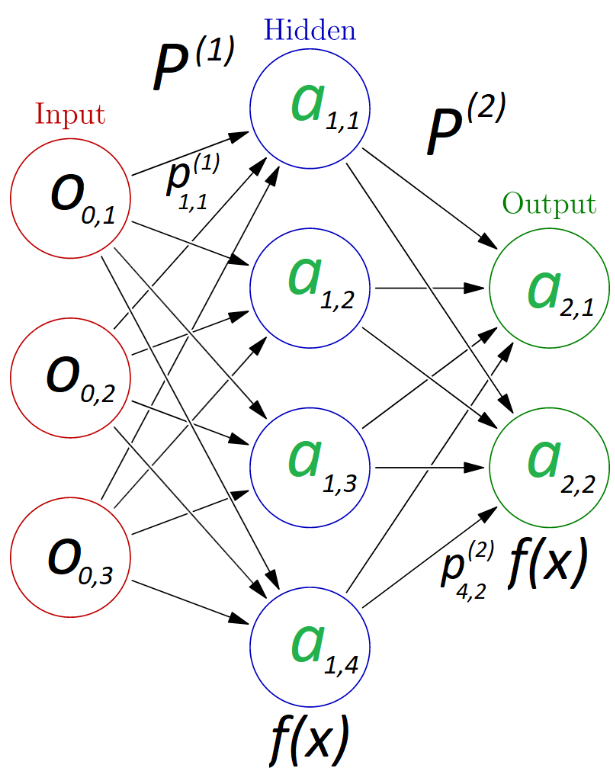
\includegraphics[totalheight=7cm]{pics/nn_1.png}
	\caption{Fully connected feedforward network}
	\label{fig:nn1}
\end{figure}

The simplest example of a neural network is a fully connected feedforward neural network. It consists of an input layer, one or more hidden layers, and an output layer. All of the neurons in the previous layer are connected with all of the neurons in the next layer. Each connection has a weight. $ P^L $ is the matrix of weights between layers $ (L - 1) $ and $ L $. The output $ o_L $ of the layer $ L $ is a column vector calculated as the product of the matrix $ P^L $ and the output of the previous layer $ o_{L-1} $. Each layer can also have an activation function $ f(x) $. Activation of the layer $ L $ is the $ a_L = f(o_L) $. Typical activation functions used are:

\vspace{4pt}
Sigmoid: \Large $ f(x) = \frac{1}{(1 - e^x)} $.
\normalsize
\vspace{4pt}

Rectified Linear Unit: $ f(x) = max(0, x) $.

Hyperbolic Tangent: \Large $ f(x) = \frac{sinh(x)}{cosh(x)} = \frac{e^x - e^{-x}}{e^x + e^{-x}}$.

\normalsize
\vspace{4pt}
The introduction of the activation functions ads nonlinearity to the input propagation through the neural network which should positively influence the accuracy of predictions.

Neural networks "learn" to make correct prediction through a process called error backpropagation\cite{13}. It allows propagating the error from the output layer to the input layer while updating the weights between the layers using gradient descent. Even though many loss functions to calculate the error have been proposed, we are going to apply classical loss function - Mean Squared Error (MSE):

\Large
$$ f(x) = \frac{\sum_{i=1}^{N} (y_{true} - y_{pred})^2}{N} $$
\normalsize

\subsection{Chosen architecture}

We propose an idea of predicting the popularity of objects in the future based on, mainly, the popularity in the past. To prepare a learning dataset, it is possible to split the request trace in time frames (or time windows) and calculate the popularity of each item in each time frame. Let’s denote this popularity as $ X_{i,j} $. Each row would consist of $ K + 1 $ popularities values, K values are input, and 1 is the output. To keep popularity independent of the number of requests in the time frame, the popularity is represented as the fraction of requests. Keeping popularity values in the "raw", unchanged state led to poor performance of the neural network since the large difference in popularity, which measured in a few orders of magnitude, caused the neural network to learn to make good predictions for the most popular objects sacrificing the accuracy of predictions of popularity for less popular objects. To fix this issue, we decided to apply a transformation for both input and output popularity values. All of the values are transformed by the next formula: $ f(p) = -log(p + const) $. This transformation reduces the difference between the smallest and the largest values processed by the neural network and proved to improve the accuracy of predictions greatly.

After some consideration, the next neural network architecture has been chosen. 4 neurons in the input layer, i. e. we are going to predict the popularity in the future based on popularity in 4 previous time frames. We will further experiment with this value discussing the performance of the proposed caching policy. Then the input is feedforwarded through 2 hidden layers with 128 neurons in each. We want to predict the popularity in the next time frame, thus only one neuron in the output layer. To every layer except the output, a bias neuron is added. A bias neuron always outputs 1 and is intended to improve the accuracy by allowing to shift the output of any layer in any dimension. As for the activation, we concluded that rectified linear unit performs the best. To overcome the "dying ReLU"\cite{14} problem, a variation of ReLU is applied - Leaky ReLU:

$$ f(x) = 
	\begin{cases}
	x, & \text{if } x \geq 0; \\
	a*x, a \ll 1 & \text{otherwise.}
	\end{cases}
$$


